% \documentclass[english, draft]{article}
\documentclass[english]{article}

%\usepackage[showframe]{geometry}
\usepackage{geometry}
\usepackage{float}
\usepackage[utf8]{inputenc}
\usepackage[backend=biber,style= authoryear]{biblatex}
% \usepackage[backend=biber]{biblatex}
\usepackage[english]{babel}
\usepackage{csquotes}
\usepackage{graphicx}
\usepackage{subcaption}
\usepackage{booktabs}

\usepackage{xargs}
\usepackage[pdftex,dvipsnames,table]{xcolor}

\graphicspath{{./resources/images}}
\addbibresource{../articles.bib}
\addbibresource{../manual.bib}

\geometry{a4paper, total={165mm,257mm}, left=15mm, top=20mm,}

\def\changemargin#1#2{\list{}{\rightmargin#2\leftmargin#1}\item[]}
\let\endchangemargin=\endlist

\title{Simultaneous phenotyping (ML approach) of sporulation and necrosis traits in the vitis spp-downy mildew interaction}
\date{22nd July 2023}
\author{
Marie-Annick Dorne, (Image acquisitions)\\
Marie-Celine Lacombe, (Pathogen, annotations review, data management)\\
Felicià Maviane, (project lead, article writing, DL and annotation)\\
Nemo Peeters (project management, article writing, pathogen),\\
Tyronne Possamai, (comparing human/machine annotations, OIV annotations)\\
David Rousseau (project management, article writing, DL)\\
Sabine Wiedemann-Merdinoglu (Project management, Article writing, Pathogen, vitis, image acquisition\\
}

\begin{document}
\pagenumbering{arabic}
\maketitle

\begin{changemargin}{60pt}{60pt}
	\begin{abstract}
		\textbf{Not abstract but overview} \newline
		\textbf{Goal(s):}
		\begin{itemize}
			\item Computer science
			      \begin{itemize}
				      \item Create method to use automatically phenotype the interaction between PV and Vitis
				      \item high throughput phenotyping
				      \item Validate the method by finding QTL in  experiments
				      \item Compare human vs machine annotation
			      \end{itemize}
			\item Biology
			      \begin{itemize}
				      \item plant breeding for mildew resistance
				      \item need to identify resistance genes in species related to the Vitis genus and in study populations
			      \end{itemize}
		\end{itemize}
		\textbf{Research or Methodology:}
		\begin{itemize}
			\item Methodology
		\end{itemize}"
		\textbf{Too many images}
            \textbf{Commentaires Nemo}
            \begin{itemize}
                \item Mettre les titres par défaut
            \end{itemize}
            \textbf{Commentaires Sabine}
            Missing bibliography
            \begin{itemize}
            	\item Velasquez-Camacho, L., Otero, M., Basile, B., Pijuan, J., Corrado, G. (2023). Current trends and perspectives on predictive models for mildew diseases in Vineyards. Microorganisms, 11, 73
            	\item Merdinoglu et al., 2018, Hogbregat et al., 2019, (A trouver dans Possamai et wiedemann\_merdinoglu, 2022)
            	\item Velasquez-Camacho et al., 2023
            \end{itemize}
            \textbf{David}
            \begin{itemize}
                \item Mat et Meth doit être neutre
                \item Zooniverse est une phrase
                \item après détailler les expériences
                \item détaillerles métriques dans mat et met
                \item les métriques uniquement dans résults
                \item regarder papiers équipe ImHorPhen dans plant methods
            \end{itemize}

	\end{abstract}
\end{changemargin}

\begin{keywords}
    Vitis, Downey Mildew, Computer vision, Deep Learning, Phenotyping, Leaf disk
\end{keywords}


\tableofcontents

\section{Introduction}

% Phenotypage imagerie important et de grands succès ref livre ou review.
% notamment en imagerie des maladies : review
% une limite est le phénotypage de symptômes/stress unique alors que dans la nature ou en conditions contrôlées souvent multiple
% On propose une approche en CNN avec un stress double pour la première fois.

% On l'applique à Vitis qui est une plante d'intérêt agronomique et économie.
% Most related work: visiion pour maladie sur vitis (liste).
% Toi tu proposes 2 symptomes traités jusqu'ici séparément dans la litérature
% Proposé avec une approche SOTA de type CNN et robots d'imagerie automatisés.

% On montre la finesse de la méthode sur des expériences historique avec QTL, on étudie les erreurs résiduels, on discute les échelles actuellement en cours, ... montrer que c'est discuté en détail.



- importance of disease world wide on vitis (ref)
- downy mildew (plasmopara viticola), details and ref, diversity ? means of controlling the disease on vitis.
- Importance of phenotyping vitis for presence of DM, for detecting Resistant cultivar in lab. phenotyping.
- outline of the article: new annotation and DL was performed on image data (already exsiting), and new DL model(s) were trained and allowed to detect simultaneously the sporulation and necroses on infected leaf discs. allowing automatic annotation of leaf discs, generating a compound OIV equivalent, and improoving the future  detection of resistant lines.


\subsection{Vitis}

\begin{figure}[H]
	\begin{center}
		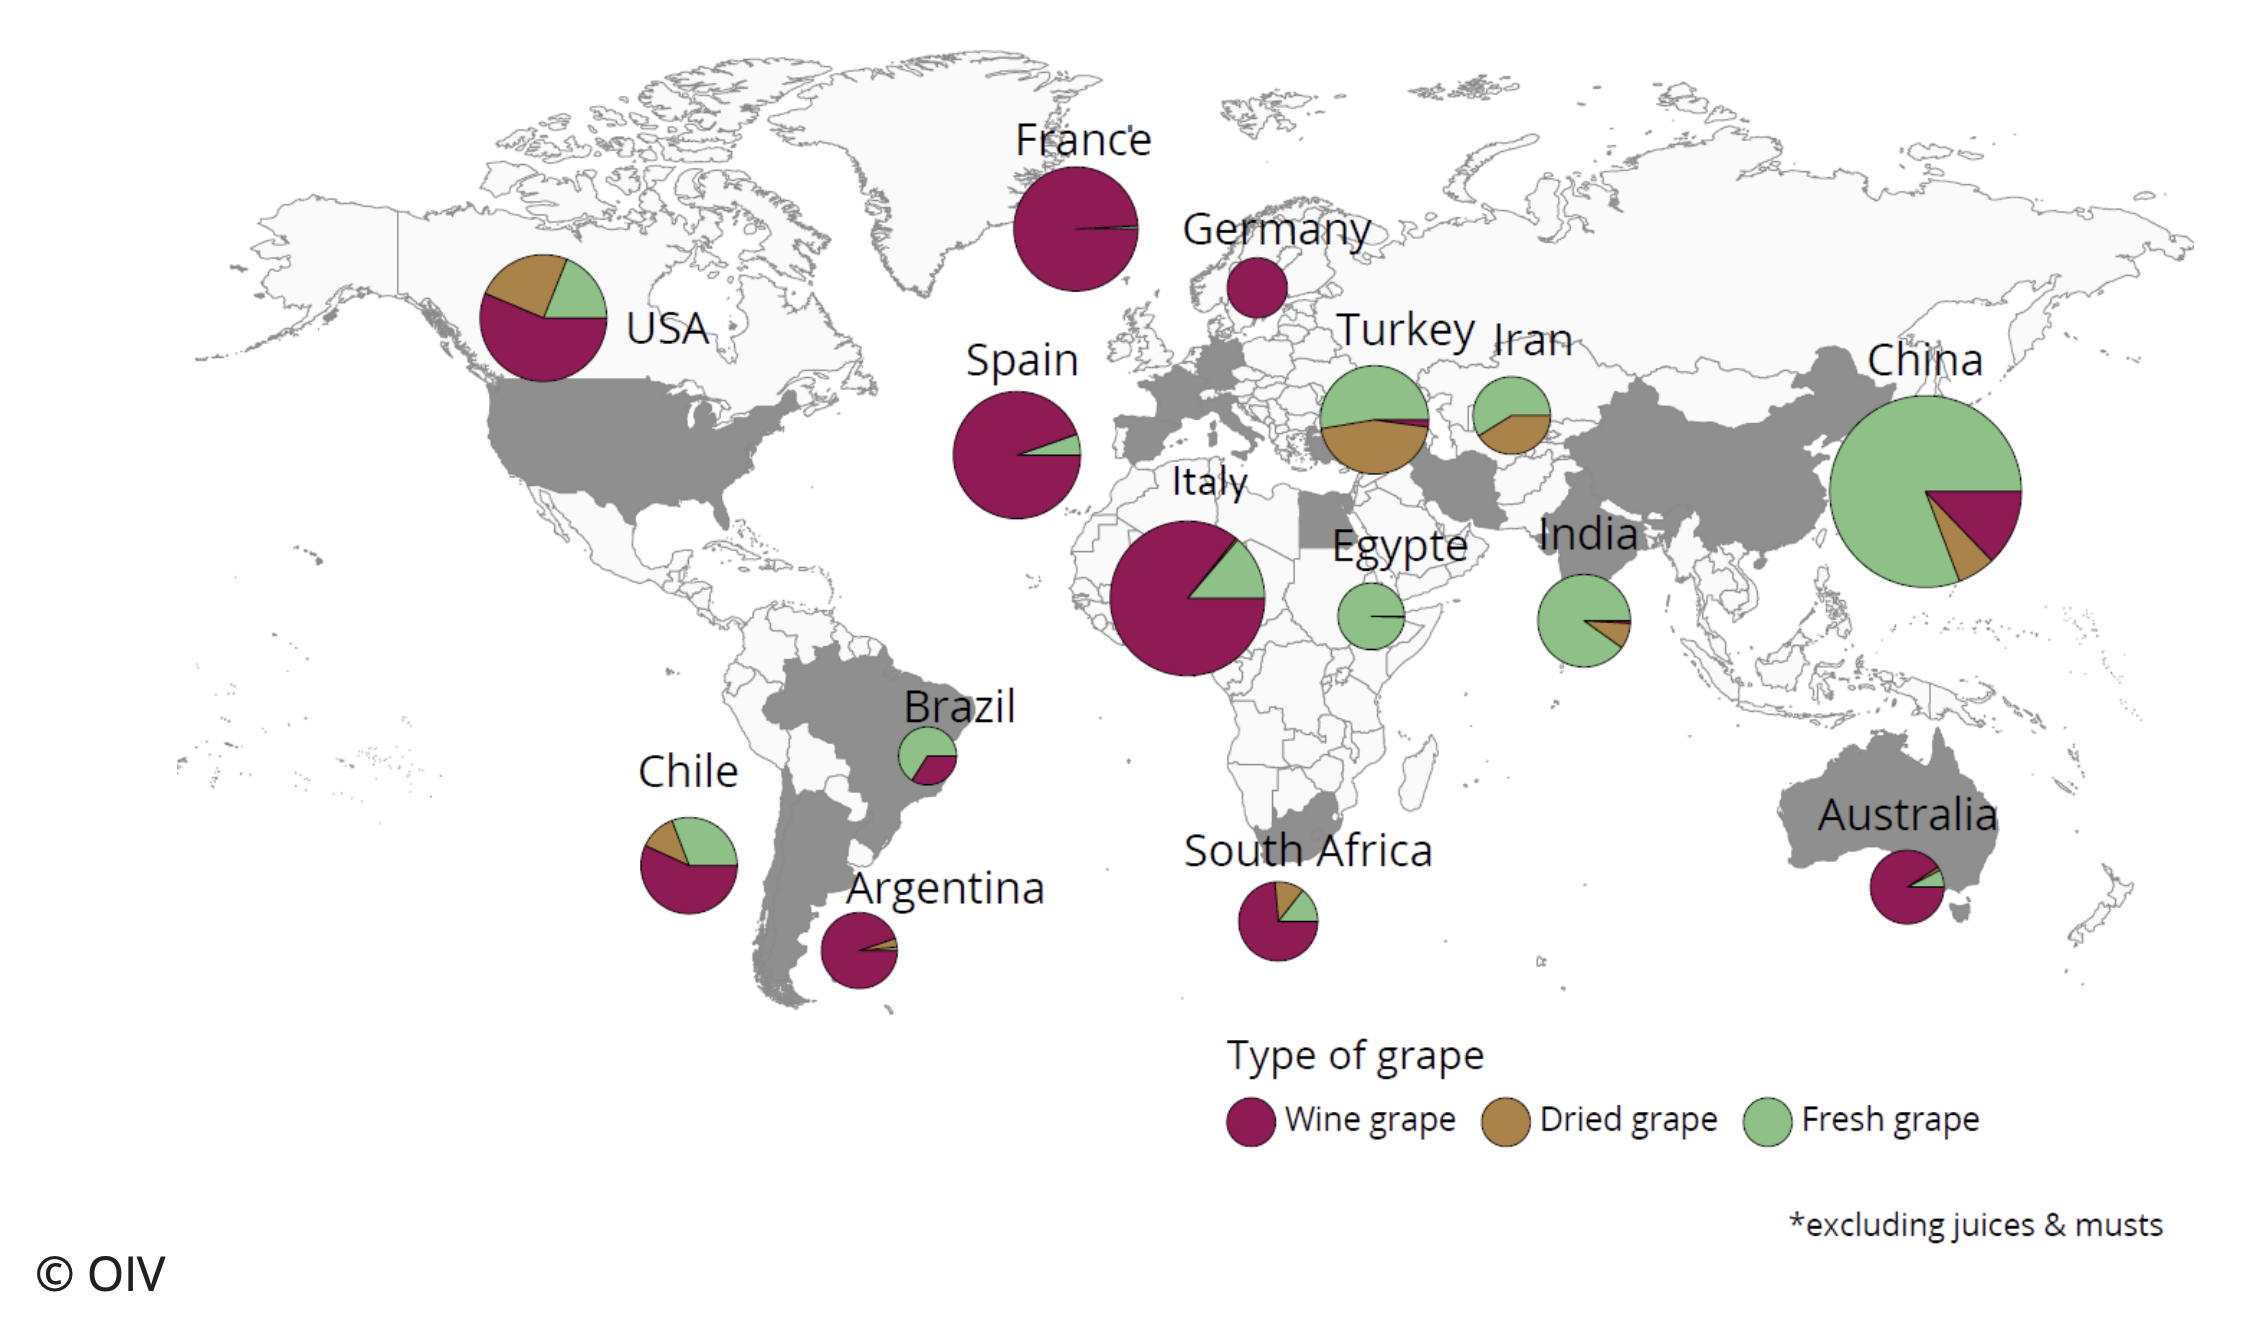
\includegraphics[width=0.7\linewidth]{2023_cdt_oiv_world.png}
		\caption{OIV nations}\label{fig:oivworld}
	\end{center}
\end{figure}

\begin{itemize}
    \item Species and their use
    \item Ancient History
    \item New threats
    \begin{itemize}
        \item Climate
        \item American pathogens $\leftarrow$
    \end{itemize}
\end{itemize}

\subsection{downy Mildew}

\begin{itemize}
	\item Description/taxonomy \textbf{velazquez}
	\item Infection mode and organ targets
	\item History~\parencite{fontaineEuropeBridgeheadWorldwide2021} \textbf{?}
	\item Consequences
	      \begin{itemize}
		      \item Yield loss
		      \item Increased use of fongicides 80\% of usage for 20\% of area (\textbf{needs citation}) $\rightarrow$
		            \begin{itemize}
			            \item Increased costs
			            \item Ecological impact
			            \item Health impact
		            \end{itemize}
	      \end{itemize}
\end{itemize}

\subsection{Existing}

\begin{enumerate}
	\item European grapevines are sensitive to American pathogens~\parencite{fontaineEuropeBridgeheadWorldwide2021}
	\item Classical breeders $\rightarrow$ poor quality wine
	\item Quality breeders after the 50s \textbf{needs citation} \textbf{?}
	\item Introduce OIV and OIV 452-1
	      \begin{itemize}
		      \item OIV = Office International de la vigne et du vin
		      \item OIV has full ontology with resistance scales
		      \item OIV 452-1 resistance to DM in leaf disks
	      \end{itemize}
	\item Critique scale \parencite{possamaiPhenotypingQTLIdentification2022}
	      \begin{itemize}
		      \item takes into account spor and necr $\rightarrow$ needs training and is complicated
		      \item plus allows comparison
		      \item nevertheless \parencite{possamaiPhenotypingQTLIdentification2022}
	      \end{itemize}
	\item Rpv3.1, Rpv10- and Rpv12 ... \textbf{needs citation} \textbf{Which ones were found with manual annotations}
	      \begin{itemize}
		      \item  \parencite{possamaiPhenotypingQTLIdentification2022} list of QTLs and how they were found
	      \end{itemize}
	\item Image processing tools \parencite{hernandezAssessmentDownyMildew2022}, \parencite{zendlerHighthroughputPhenotypingLeaf2021}
\end{enumerate}

\subsection{Novelty}

\begin{itemize}
	\item Current computer vision approaches only look at sporulation
	\item Our approach looks at sporulation plus 3 types of necrosis \textbf{necrosis as important as sporulation?}
	\item \textbf{TODO} \textbf{Goal}: Predict OIV 452-1 from images for binary variables
	\item \textbf{TODO} Test on existing experiments
\end{itemize}

\section{Materials and Methods}

\subsection{Plants}

\parencite{bellinResistancePlasmoparaViticola2009} \textbf{new version needed}

\subsection{Infection}

\parencite{bellinResistancePlasmoparaViticola2009}

\subsection{Image acquisition}

\begin{itemize}
	\item Acquisitions since 2018
	\item Multiple acquisition Methods != camera, lenses, lightning, framing, compression, post processing $\rightarrow$ needs additional work to exploit the data \textbf{Why not use simple approach?}
	\item Plates
\end{itemize}

\subsection{Existing data overview}

\begin{figure}
	\begin{center}
		\includegraphics[width=0.7\linewidth]{oiv_452-1_desc.png}
		\caption{Additional variables}\label{fig:newvariables} \textbf{To be replaced by text}
	\end{center}
\end{figure}

\begin{itemize}
	\item Database structure: Excels + images in folders with experiment metadata
	\item OIV and additional variables
	      \begin{itemize}
		      \item OIV 452-1
		      \item New variables~\ref{fig:newvariables}
	      \end{itemize}
	\item $\rightarrow$ Excel to CSV
	\item Naive prediction
	      \begin{itemize}
		      \item LDA, random forrest
		      \item fail~\ref{fig:predictionfail} means that additional variables are not able to predict OIV, but they still may have signal
		      \item multiple OIV values per combination~\ref{tab:oivconfusion}
	      \end{itemize}
\end{itemize}

\begin{figure}[H]
	\begin{center}
		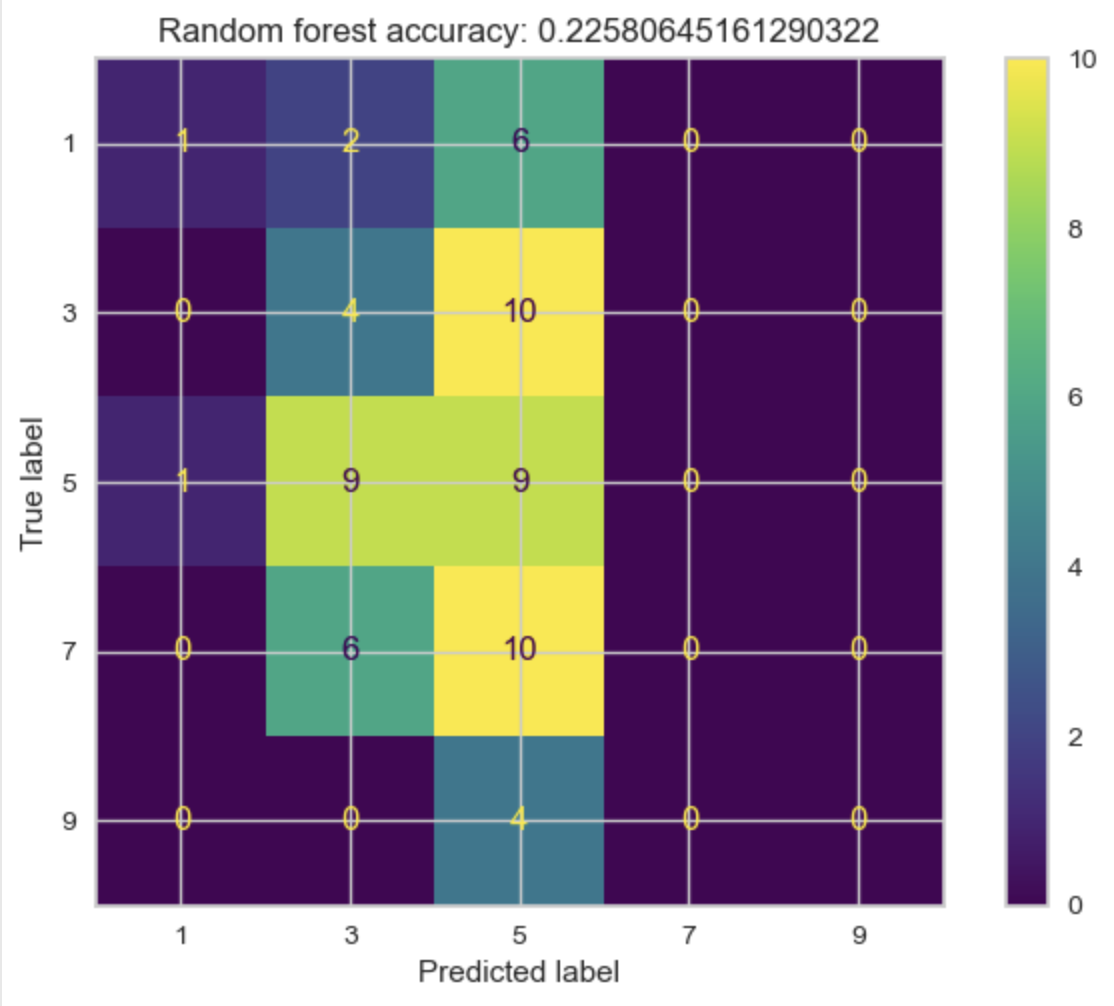
\includegraphics[width=0.7\linewidth,trim={1mm 0 0 0},clip]{annotations_da_rfc_cm.png}
		\caption{Prediction fail}\label{fig:predictionfail}
	\end{center}
\end{figure}

\paragraph{Fig: \ref{fig:predictionfail} Prediction fail}
Can we predict OIV 452-1 from additional variables? NO, an accuracy of 0.226 shows model is close to random

\begin{table}[H]
	\centering
	\caption{OIV row multi-value}\label{tab:oivconfusion}
	\begin{tabular}{rrrrrccccc}
		\toprule
		sporulation & sporulation & necrosis & necrosis & necrosis & oiv 1 & oiv 3 & oiv 5 & oiv 7            & oiv 9 \\
		{}          & density     & {}       & size     & area     & {}    & {}    & {}    & {}               & {}    \\
		\midrule
		1           & 1           & 0        & 1        & 1        & X     & X     & X     & X                &       \\
		1           & 7           & 1        & 3        & 5        & X     & X     & X     & X                &       \\
		1           & 5           & 1        & 9        & 9        & X     & X     & X     & X                &       \\
		1           & 5           & 1        & 1        & 7        &       &       & X     & X                &       \\
		1           & 1           & 1        & 3        & 1        &       &       & X     & X                &       \\
		0           & 1           & 1        & 3        & 3        &       &       &       & X \textbf{ERROR} & X     \\
		\bottomrule
	\end{tabular}
\end{table}
\paragraph{Fig:~\ref{tab:oivconfusion} OIV confusion}
\begin{itemize}
	\item Is there a reason for the model to fail prediction? Same combination of variables can yield the multiple OIVs
	\item \textbf{Remaining error in data} All OIVs other than 9 should have sporulation, check data filtering
\end{itemize}


\subsection{Leaf Extraction}

\begin{itemize}
	\item Ilastik~\parencite{bergIlastikInteractiveMachine2019} fail because extremely different images
	\item U-Net~\parencite{ronnebergerUNetConvolutionalNetworks2015} misses some leaf discs in corner cases
	\item Fast R-CNN~\parencite{girshickFastRCNN2015}
	\item Indexation
	\item Patch extraction~\ref{fig:patchextraction}
\end{itemize}


\begin{figure}[H]
	\centering
	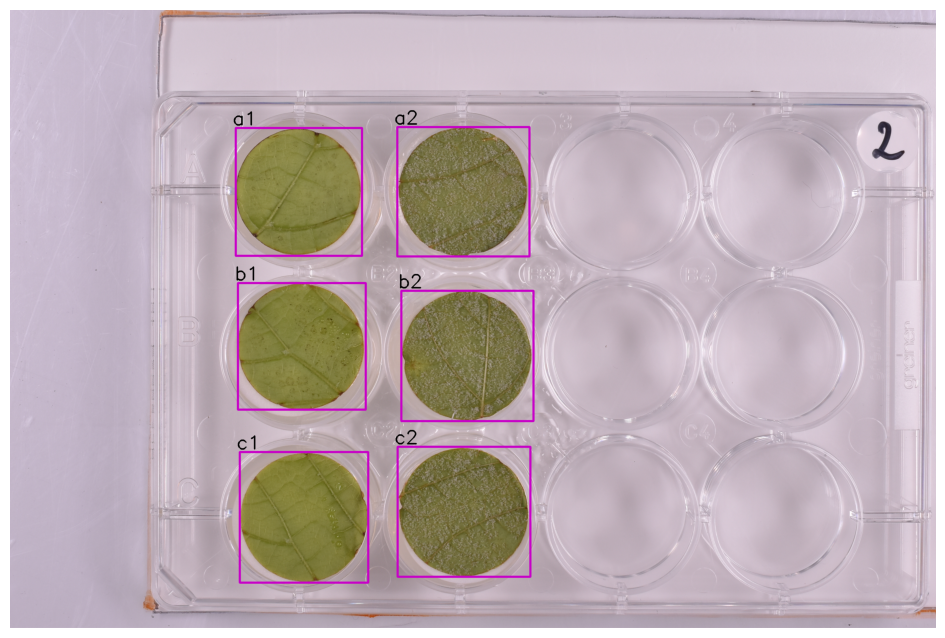
\includegraphics[width=0.8\linewidth]{plate_index_v2_fixed.png}
	\caption{Leaf disc detect}\label{fig:plateindexation}
\end{figure}

\paragraph{Fig:~\ref{fig:plateindexation} plate indexation}
\begin{itemize}
	\item Steps to extract and index leaf discs
	\item Why not stay with Ilastik?: too many variations in image acquisitions
	\item \textbf{Add image more representative of various steps needed to index and the difficulties faced}
\end{itemize}

\begin{figure}[H]
	\centering
	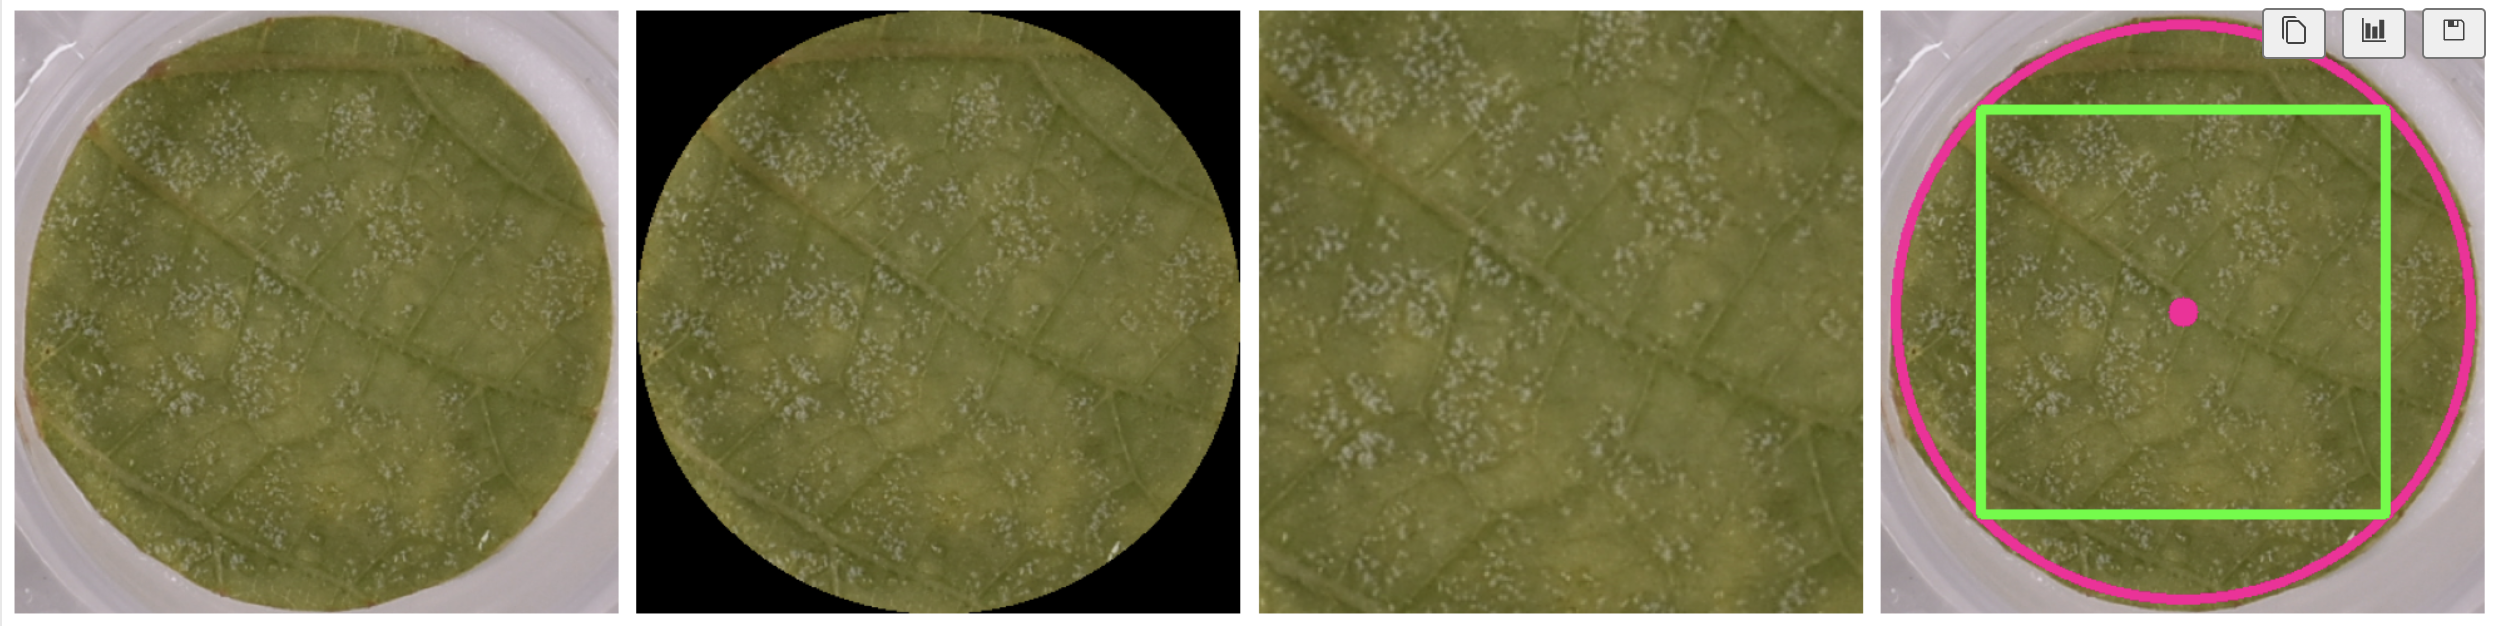
\includegraphics[width=0.8\linewidth]{ld_detector_brute_force.png}
	\caption{Patch extraction}\label{fig:patchextraction}
\end{figure}

\paragraph{Fig:~\ref{fig:patchextraction} Patch Extraction}
\begin{itemize}
	\item Why square?: to prevent the model to look at the background.
	\item Are we missing data?: Square represents over 82\% of the leaf disc
\end{itemize}

\textbf{Talk about failed approaches?}

\subsection{Binary prediction}
Zooniverse \parencite{zooniverse}

\textbf{Add set construction to methodo}

\begin{itemize}
	\item online annotation platform
	\item Multiple annotations per disc
\end{itemize}

\subsubsection{Image Annotation}

\begin{figure}[H]
	\centering
	\begin{subfigure}[b]{0.2\linewidth}
		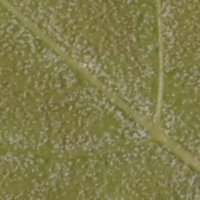
\includegraphics[width=\linewidth]{Exp21DM01_inoc1_T6_P24_c_2.png}
		\caption{Sporulation}\label{fig:sporulation}
	\end{subfigure}
	\begin{subfigure}[b]{0.2\linewidth}
		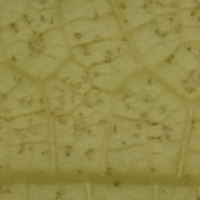
\includegraphics[width=\linewidth]{Exp20DM01_inoc1_T6_P17_c_1.png}
		\caption{Necrosis spots}\label{fig:necrosisspots}
	\end{subfigure}
	\begin{subfigure}[b]{0.2\linewidth}
		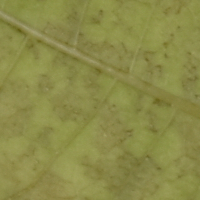
\includegraphics[width=\linewidth]{Exp20DM01_inoc2_T6_P47_c_4.png}
		\caption{Necrosis flecks}\label{fig:necrosisstains}
	\end{subfigure}
	\begin{subfigure}[b]{0.2\linewidth}
		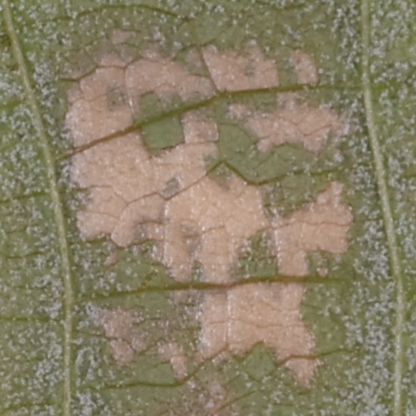
\includegraphics[width=\linewidth]{Exp21DM04_inoc2_T6_P12_a_3.png}
		\caption{Necrosis senescence}\label{fig:necrosissenescence}
	\end{subfigure}
	\caption{The Four Phenotypes}\label{fig:phenotypes}
\end{figure}

\paragraph{Fig:~\ref*{fig:phenotypes} Four phenotypes}
\begin{itemize}
        \item \textbf{Why:} Supposed to be easier to annotate than OIV 452-1 cf. OIV critique
	\item Describe individual phenotypes
	\item Why THIS 4?: We hope they represent the possible variation of the effect of the pathogen and the responses of the plant. Sporulation only represents the fitness of the pathogen \textbf{Needs checking and citation}
\end{itemize}

\begin{table}[H]
	\caption{Zooniverse V1 data}\label{tab:zv1data}
	\begin{minipage}{0.4\linewidth}
		% \centering
		\caption{Class cardinals}\label{tab:zoonv1classcardinals}
		\begin{tabular}{rc}
			\toprule
			Phenotype           & Count \\
			\midrule
			sporulation         & 757   \\
			necrosis spots      & 247   \\
			necrosis flecks     & 149   \\
			necrosis senescence & 50    \\
			\bottomrule
		\end{tabular}
	\end{minipage}%
	\begin{minipage}{0.4\linewidth}
		\centering
		\caption{Classification report}\label{tab:zv1mcr}
		\begin{tabular}{rcccc}
			\toprule
			{}                                    & Precision & Recall & F1 score & Support \\
			\midrule
			sporulation                           & 0.92      & 0.93   & 0.93     & 113     \\
			necrosis spots                        & 0.82      & 0.38   & 0.52     & 37      \\
			\rowcolor{red!25} necrosis flecks     & 0.00      & 0.00   & 0.00     & 22      \\
			\rowcolor{red!25} necrosis senescence & 0.00      & 0.00   & 0.00     & 8       \\
			micro avg                             & 0.91      & 0.66   & 0.77     & 180     \\
			macro avg                             & 0.44      & 0.33   & 0.36     & 180     \\
			weighted avg                          & 0.75      & 0.66   & 0.69     & 180     \\
			\bottomrule
		\end{tabular}
	\end{minipage}
\end{table}

\paragraph{Tab:~\ref{tab:zv1data} First Zooniverse annotations and model}
\begin{itemize}
	\item \textbf{Why this many images?} lots for scratch model 10000 for transfer learning, 1000 with data augmentation
	\item \textbf{Dataset creation?} Naive sample of 1000 images from 80k available
	\item \textbf{Annotation}: Zooniverse
	\item \textbf{Model caracteristics?}~\parencite{dosovitskiyImageWorth16x162021} and others
	\item \textbf{Hyperparameters} get form notebooks
	\item \textbf{Issue}: Bad class cardinals repartition
	\item \textbf{Issue}: Some low quality images got through
\end{itemize}

\begin{table}[H]
	\caption{Zooniverse V2 data}\label{tab:zv2data}
	\begin{minipage}{0.4\linewidth}
		\centering
		\caption{Class cardinals}\label{tab:zoonv2classcardinals}
		\begin{tabular}{rc}
			\toprule
			Phenotype           & Count \\
			\midrule
			sporulation         & 1188  \\
			necrosis spots      & 578   \\
			necrosis flecks     & 467   \\
			necrosis senescence & 271   \\
			\bottomrule
		\end{tabular}
	\end{minipage}%
	\begin{minipage}{0.4\linewidth}
		\centering
		\caption{Classification report}\label{tab:zv2mcr}
		\begin{tabular}{rcccc}
			\toprule
			{}                   & precision & recall & f1-score & support \\
			\midrule
			sporulation          & 0.9922    & 0.9078 & 0.9481   & 141     \\
			necrosis\_spots      & 0.9388    & 0.8679 & 0.9020   & 106     \\
			necrosis\_stains     & 0.7313    & 0.7656 & 0.7481   & 64      \\
			necrosis\_senescence & 0.6800    & 0.8947 & 0.7727   & 38      \\
			micro avg            & 0.8808    & 0.8682 & 0.8745   & 349     \\
			macro avg            & 0.8356    & 0.8590 & 0.8427   & 349     \\
			weighted avg         & 0.8942    & 0.8682 & 0.8783   & 349     \\
			\bottomrule
		\end{tabular}
	\end{minipage}
\end{table}

\paragraph{Tab:~\ref{tab:zv1data} First Zooniverse annotations and model}
\begin{itemize}
	\item \textbf{Dataset creation?} Piecewise sample to obtain balanced class cardinals
	\item \textbf{Annotation}: Zooniverse
	\item \textbf{Why this many images?} Target was 1000 images, piecewise sampling yielded more
	\item \textbf{Model caracteristics?}~\parencite{dosovitskiyImageWorth16x162021} and others
	\item \textbf{Hyperparameters} get form notebooks
	\item \textbf{Issue}: Bad class cardinals repartition -- fixed but not perfect
	\item \textbf{Issue}: Some low quality images got through -- Still some bad images
	\item \textbf{Issue}: More varied images == more complicated images => annotation disparities
\end{itemize}

\textbf{Annotation rounds used to show human error} -- \textbf{?}
\textbf{Are all annotation rounds and models needed? Or only discuss shortcommings}

\subsubsection{Model}


\begin{itemize}
	\item \textbf{Dataset creation?} Piecewise sample to obtain balanced class cardinals, kept bad images. images were tagged with quality information
	\item \textbf{Annotation}: Experts only by agreement
	\item \textbf{Why this many images?} Target was 1000 images, piecewise sampling yielded more (1881)
	\item \textbf{Model caracteristics?}~\parencite{dosovitskiyImageWorth16x162021} and others
	\item \textbf{Hyperparameters} get form notebooks
	\item \textbf{Issue}: Bad class cardinals repartition -- fixed but not perfect -- Improved
	\item \textbf{Issue}: Some low quality images got through -- Still some bad images -- Annotated => more images better than good images only
	\item \textbf{Issue}: More varied images == more complicated images $\rightarrow$ annotation disparities $\rightarrow$ experts only
\end{itemize}

\begin{table}[H]
	\caption{New patches data}
	\begin{minipage}{0.4\linewidth}
		\centering
		\caption{Class cardinals}\label{tab:imprpatchersclassdistribution}
		\begin{tabular}{rc}
			\toprule
			Phenotype           & Count \\
			\midrule
			sporulation         & 1119  \\
			necrosis dots       & 712   \\
			necrosis flecks     & 289   \\
			necrosis senescence & 444   \\
			\bottomrule
		\end{tabular}
	\end{minipage}%
	\begin{minipage}{0.4\linewidth}
		\centering
		\caption{Classification report}\label{tab:imprpatches4phenotypes}
		\begin{tabular}{rcccc}
			\toprule
			{}                  & Precision & Recall & F1 score & Support \\
			\midrule
			sporulation         & 0.96      & 0.94   & 0.95     & 156     \\
			necrosis dots       & 0.86      & 0.82   & 0.84     & 90      \\
			necrosis flecks     & 0.82      & 0.90   & 0.86     & 41      \\
			necrosis senescence & 0.93      & 0.89   & 0.91     & 57      \\
			micro avg           & 0.91      & 0.90   & 0.90     & 344     \\
			macro avg           & 0.89      & 0.89   & 0.89     & 344     \\
			weighted avg        & 0.91      & 0.90   & 0.90     & 344     \\
			\bottomrule
		\end{tabular}
	\end{minipage}
\end{table}

\begin{figure}[H]
	\centering
	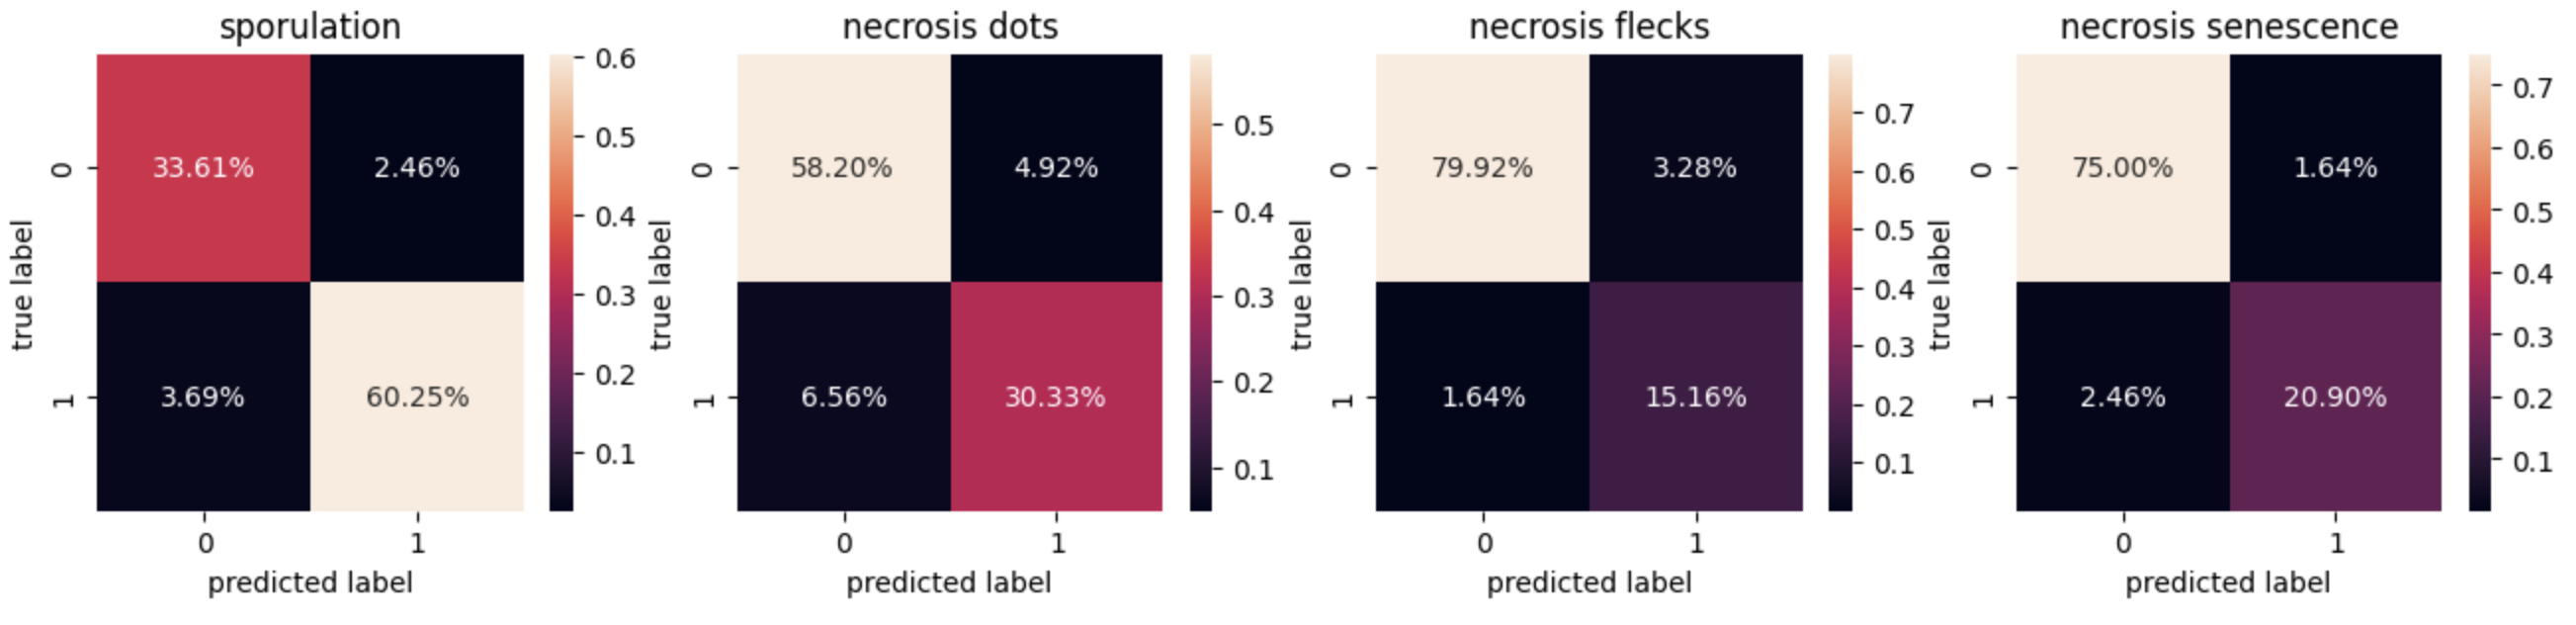
\includegraphics[width=0.8\linewidth]{p_viticola/2023_cdt_best_model_cm.png}
	\caption{Confusion matrix for best model}\label{fig:cmbestmodel}
\end{figure}

\paragraph{Fig:~\ref{fig:cmbestmodel} Confusion matrix for best model}
\begin{itemize}
    \item Model shows good results
    \item phenotypes that were hard to annotate exhibit the worst scores
\end{itemize}

\begin{figure}[H]
	\centering
	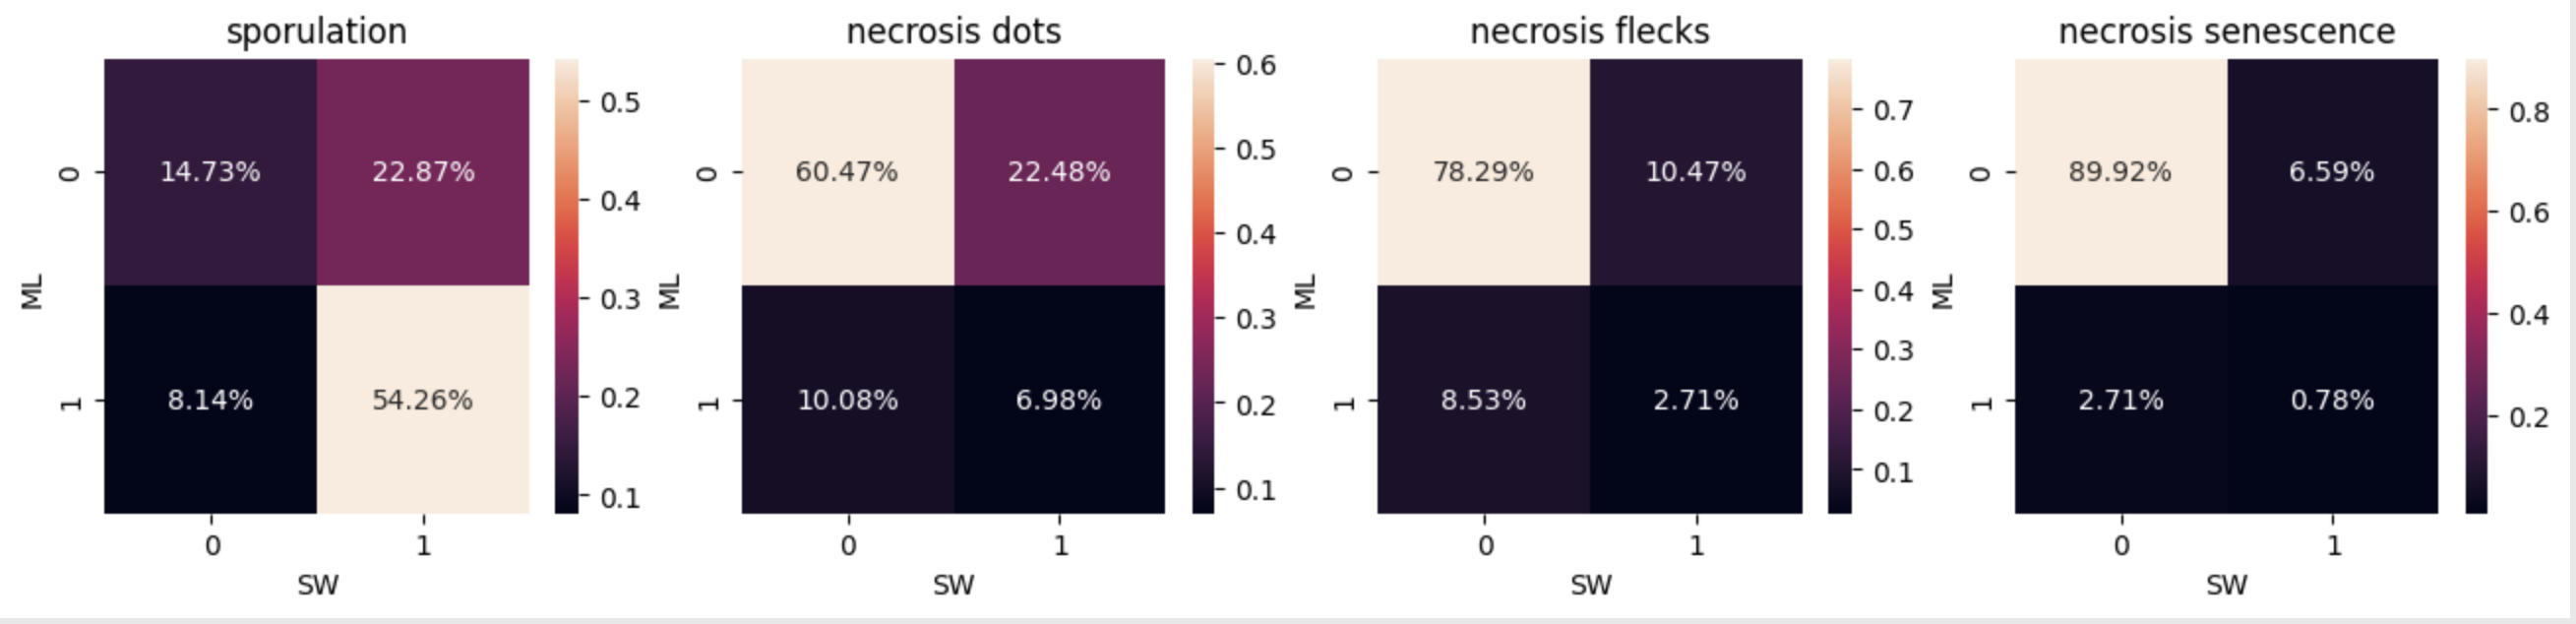
\includegraphics[width=0.8\linewidth]{p_viticola/2023_cdt_experts_cm.png}
	\caption{Confusion matrix for experts annotations}\label{fig:cmexpanno}
\end{figure}

\paragraph{Fig:~\ref{fig:cmexpanno} Experts annotations comparison}
\begin{itemize}
    \item Experts are less consistent than model
\end{itemize}

\begin{figure}[H]
	\centering
	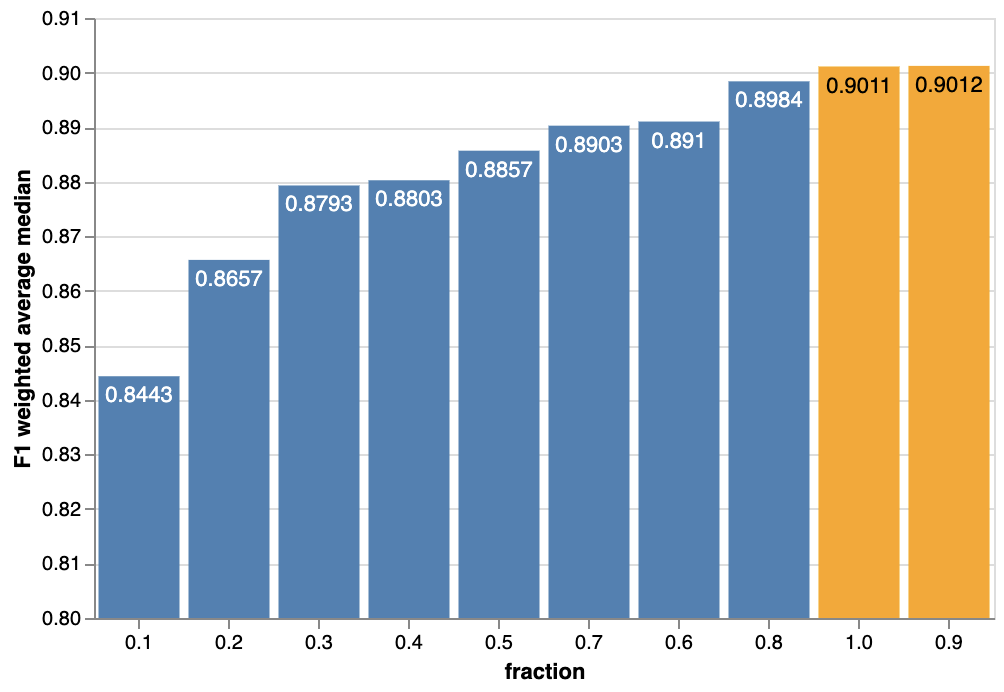
\includegraphics[width=0.8\linewidth]{2023_cdt_data_frac_evolution.png}
	\caption{Ablation tests}\label{fig:ablationtests}
\end{figure}

\paragraph{Fig:~\ref{fig:ablationtests} Ablation tests}
\begin{itemize}
	\item from 10\% to 100\% of dataset improvement of 0.05 in f1 score
	\item plateau?
	\item Add more images?
\end{itemize}

\begin{itemize}
	\item pytorch + pytorch lightning
	\item based on~\parencite{dosovitskiyImageWorth16x162021} and others
	\item training hyperparameters
	\item training steps
	\item ablation tests
\end{itemize}

\begin{figure}[H]
	\centering
	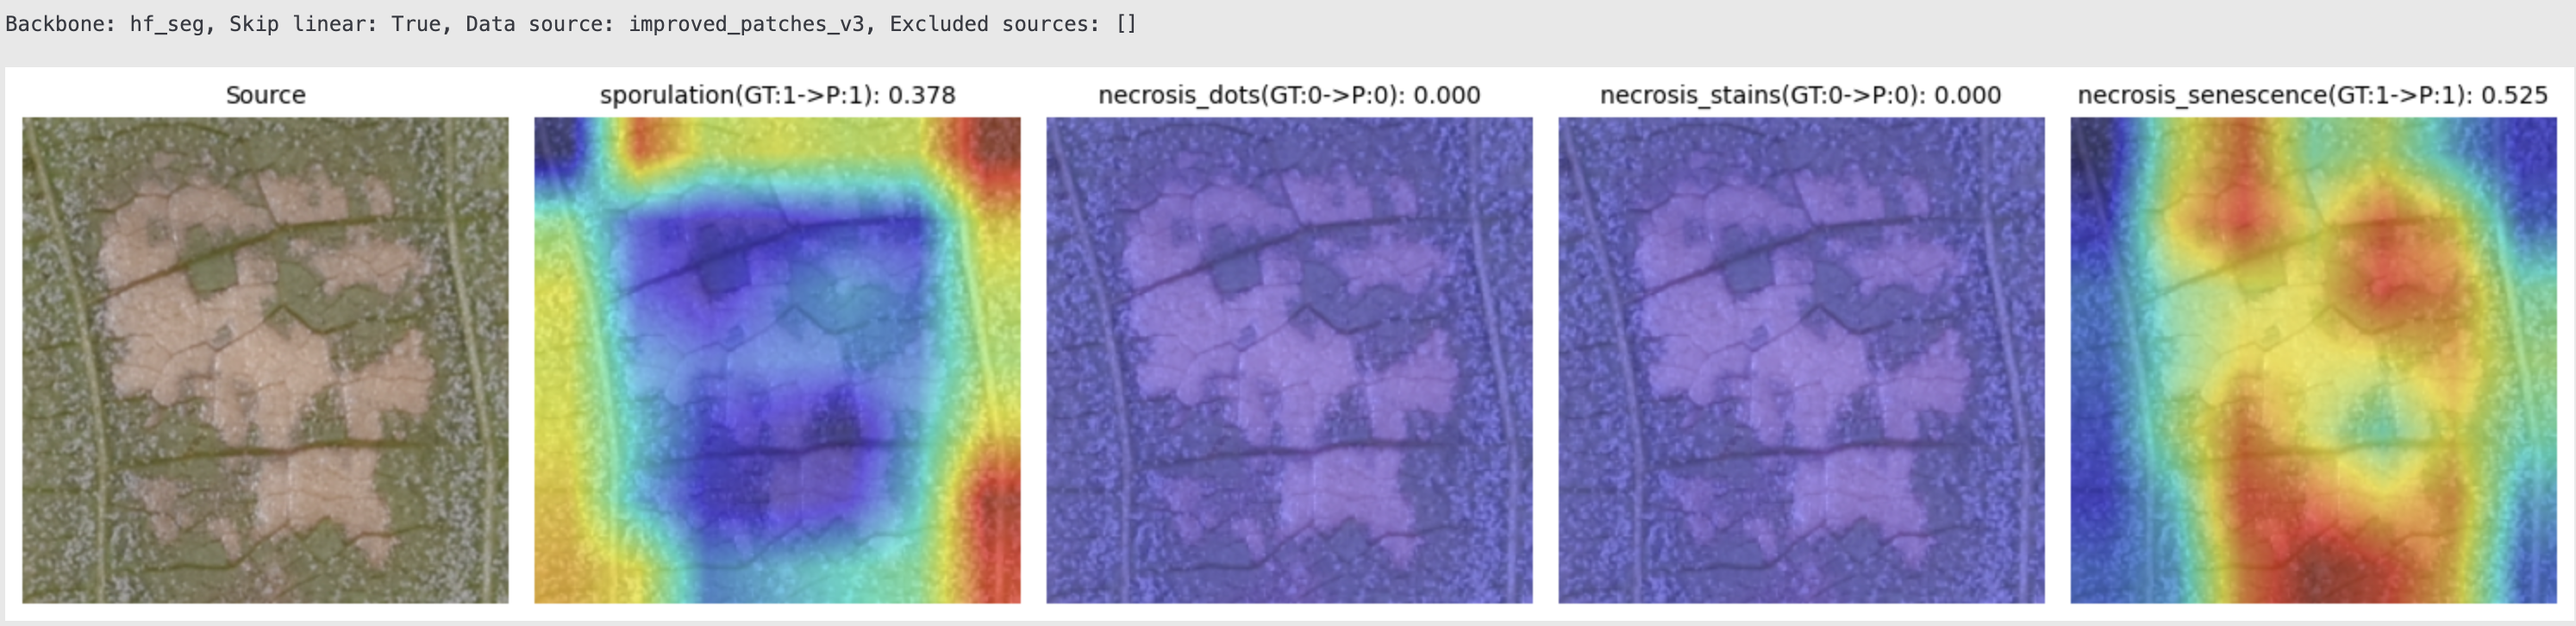
\includegraphics[width=0.8\linewidth]{gc_hf_seg_sen_high.png}
	\caption{Grad-CAM validation}\label{fig:gradcamval}
\end{figure}

\paragraph{Fig:~\ref{fig:gradcamval}}
\begin{itemize}
	\item Grad-CAM used for visual validation of binary model
\end{itemize}

\subsection{OIV 452-1 prediction}

Why create a new model instead of using the binary predictions
\begin{itemize}
    \item Binary predictions lack enough information
    \item It appears that the 4 variables are as complicated to annotate as the OIV
\end{itemize}

\begin{itemize}
	\item Annotation of 1881 leaf discs with OIV 452-1
	\item Independent binary scales not enough to predict QTLs (will be tried t be sure)
	\item Use binary predictions + image data to create a scale to feed to the QTL research
	\item Multiple options for scale
	      \begin{itemize}
		      \item OIV 452-1
		      \item Create new scale \textbf{Possible approach: Use dimensional reduction techniques to check if some types of leaves are clustered}
		      \item Discrete or continuous?
	      \end{itemize}
	\item Validate method by analyzing previous known experiments
	\item \textbf{Additional:} Compare human/computer annotations at different dai to see differencies in correlation by date
\end{itemize}

\textbf{Availabe:}
\begin{itemize}
	\item Annotations of 1881 leaf discs
\end{itemize}
\textbf{Missing:}
\begin{itemize}
	\item Annotation review
	\item Predictive model, discrete?
	\item Analyze previous experiments
\end{itemize}

\subsection{Experiments re-analysis}

\section{Results}

Global DM phenotype on Vitis as factor of 4 discrete traits



\subsection{Unreliable human factor \textbf{?}}

\subsection{Binary prediction as a heuristic for scale prediction}

\subsection{Result from experiment re-analysis}


\section{Discussion}



% \clearpage
\printbibliography

\end{document}

